\documentclass{article}
\usepackage{graphicx}
\usepackage[utf8]{inputenc}
\usepackage{hyperref}

\begin{document}
\begin{titlepage}
	\centering
	\includegraphics[width=0.15\textwidth]{utec}\par\vspace{1cm}
	{\scshape\LARGE Developer Guide \par}
	\vspace{0.5cm}
	{\scshape\Large Yacket\par}
	\vspace{0.5cm}
	{\huge\bfseries Ingeniería de software\par}
	\vspace{1.0cm}
	{\Large\itshape Antonio Toche\par}
	\href{mailto:antonio.toche@utec.edu.pe}{antonio.toche@utec.edu.pe}\\
	\vspace{1.0cm}
	{\Large\itshape Sergio Carbone\par}
	\href{mailto:sergio.carbone@utec.edu.pe}{sergio.carbone@utec.edu.pe}\\
	\vspace{1.0cm}
	{\Large\itshape Jeffrey Orihuela\par}
	\href{mailto:sergio.carbone@utec.edu.pe}{jeffrey.orihuela@utec.edu.pe}\\
	\vspace{1.0cm}
	{\Large\itshape José Chávez\par}
	\href{mailto:jose.chavez@utec.edu.pe}{jose.chavez@utec.edu.pe}\\
	\vspace{1.0cm}
	{\Large\itshape Fernando Socualaya\par}
	\href{mailto:fernando.socualaya@utec.edu.pe}{fernando.socualaya@utec.edu.pe}\\
	\vspace{1.0cm}
	\vfill
	Profesores\par
	Jesús Bellido\\
	Yamilet Serrano\\
	\vfill
	{\large \today\par}
\end{titlepage}

\section{Introduction}
Since the evolution of the internet and the creation of smart phones, mobile applications have become increasingly necessary to facilitate us in our daily lives. In banking issues this facility is not alien, since the way to transfer money has changed radically. One of the applications that most sound and have changed the way we do transactions is Yape, this is an application for smarthphones launched by the BCP that facilitates the transfer of money.
 In the course of Software Engineering a professional environment has been recreated with real costumers, in this case Yape is the costumer to whom we have to advise so that the number of users that he has increases rapidly, for which he will have to present an idea for then validate it and, followed by the metrics taught in the course, implement them. In the present report, Yacket will be presented which will add the feature of issuing an electronic invoice to the Yape application, in this way we intend to increase the amount of Yaperos.
For this, two potential costumers have been defined. The first one is the yape costumer that usually goes to mypes and pymes. The second is a possible owner and owner of the mypes and pymes. Both like technology and constantly seek new ways to digitize the entire sales process, taking advantage of these tools that speed up, ensure and facilitate buying and selling.
The purpose of this project will be to implement the functionality of electronic tickets and invoices through Yape.

\section{Features}
 \subsection{Antonio Toche/Fernando Socualaya/Sergio Carbone: UI design}
 \blindtext
\subsubsection{Sergio Carbone/Antonio Toche/Fernando Socualaya: Yape UI}
This section will recreate the UI of the yape application since our functionality will be within the same application. Thanks to the enhanced interviews, it was decided that the functionality will be done within the application, so it is necessary to recreate the Yape interface (see Annex A).
\begin{itemize}
\item v1.1 Add login UI.
\item v1.2 Add Main page UI.
\item v1.3 Add sidebar.
\item v1.4 Add componentes.
\end{itemize}

\subsubsection{Sergio Carbone: Entity picker}
In this section you can select if it is a company or an User. Since to generate a bill / invoice you need to be a company.(see Annex B).
\begin{itemize}
\item v1.1 Add button component.
\item v1.2 Add pickers.
\end{itemize}

\subsubsection{Sergio Carbone: Person pay feature}
To try to recreate Yape as best as possible, it is necessary to integrate the interfaces it has.
\begin{itemize}
\item v1.1 Add person pay feature interface.
\item v1.2 Add forms.
\item v1.3 Add button to pay.
\end{itemize}

\subsubsection{Sergio Carbone: Add business info}
We need to save the business data for invoices purpose.
\begin{itemize}
\item v1.1 Add forms.
\item v1.3 Add button to save.
\end{itemize}

\subsubsection{Antonio Toche: Business pay feature}
In this section the items are placed to later collect. It is working in this way since it is necessary to set aside this method of payment with what a client normally does.(See Anexx C)
\begin{itemize}
\item v1.1 Add business pay feature interface.
\item v1.2 Add forms.
\item v1.3 Add buttons to get/change new business.
\end{itemize}

\subsubsection{Fernando Socualaya: Qr code feature}
Once the items are placed, you will need to generate the Qr code so that the payment can be made effectively.(See anexx D)
\begin{itemize}
\item v1.1 Add Qr interface.
\end{itemize}

 \subsection{Antonio Toche/Fernando Socualaya/Sergio Carbone/Jose Chavez/ Jeffrey Orihuela: Implementation}
 \blindtext
\subsubsection{Jeffrey Orihuela/Antonio Toche: Ticket}
The ticket generator will be the feature that sends the generated ticket to the respective emails. For this feature, you need the yape owner's email and the customer's email these had to be filled in previously.
\begin{itemize}
\item v1.1 Get data.
\item v1.2 Send email.
\item v1.3 Save ticket.
\end{itemize}

\subsubsection{Fernando Socualaya/José Chavez: Bill}
The selling generator will be the component that sends the generated selling to the respective emails. For this function, you need the email from the Yape owner and the customer's email, in addition you will need the Ruc, all these had to be filled in previously.
\begin{itemize}
\item v1.1 Get data.
\item v1.2 Send data to reniec.
\item v1.3 Send/Save bill to email.
\end{itemize}

\subsubsection{Sergio Carbone/Jeffrey Origuela: Qr generator}
Once the items are placed, you will need to generate the Qr code so that the payment can be made effectively.
\begin{itemize}
\item v1.1 Get/Show data.
\item v1.2 Set Qr.
\end{itemize}
\section{Design}
\subsection{Architecture}
\subsubsection{Class Diagram}
\subsubsection{Architecture Diagram}
\subsubsection{Components}
\subsubsection{Interaction between components}
\section{FAQ}
\section{Glossary}
\begin{itemize}
    \item Yape: name of the application.
    \item Yacket: name of the services.
    \item MYPE/PYME: Micro and Small sized enterprises.
    \item Micro sized entreprise: Conformed by less than 10 employees.
    \item Client: person who use yape to pay.
    \item Small sized entreprise: Conformed by less than 20 employess.
    \item Consumer: The person who purchase a product.
    \item MYPE/PYME owner: The person who owns/manages a MYPE/PYME.
    \item Ticket/invoice/selling: Payment vouchers.
    \item SUNAT: Entity that collects taxes.
\end{itemize}
\section{Anexos}
\subsection{A}
\\In an interview with owners / managers and cashiers of a business, one of the questions taken into account was:\\\\\\
\includegraphics[width=1\textwidth]{inside}\par\vspace{1cm}

\subsection{B}
Part of the Mockup to recreate the entity picker:\\\\\\
\includegraphics[width=0.5\textwidth]{entity}\par\vspace{1cm}
	\vspace{2.0cm}
\subsection{C}
Business forms:\\\\
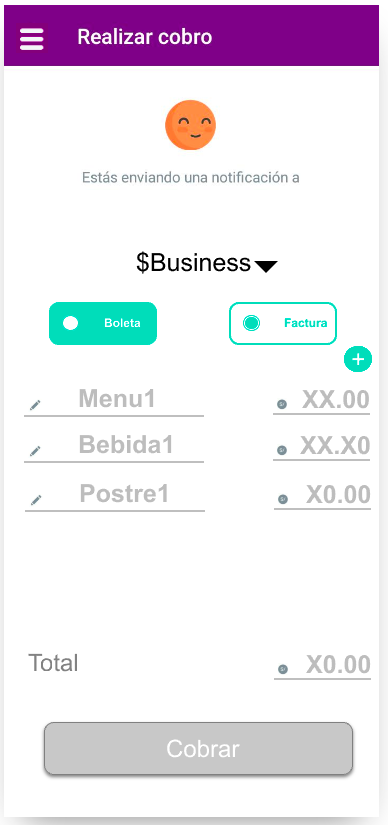
\includegraphics[width=0.5\textwidth]{factura}\par\vspace{1cm}
	\vspace{2.0cm}

\subsection{D}
Qr generator:\\\\
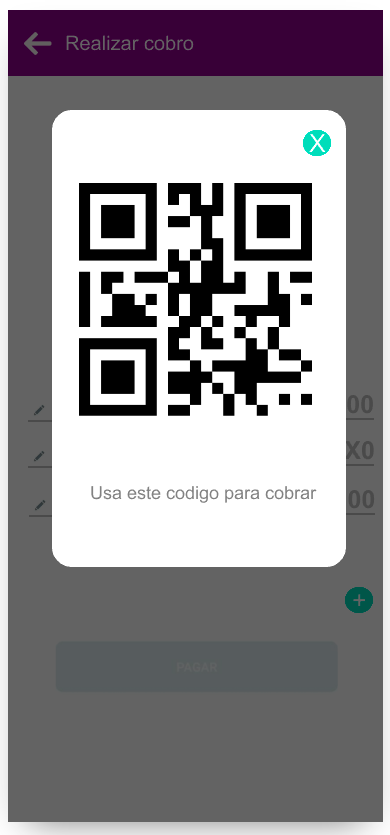
\includegraphics[width=0.5\textwidth]{qr}\par\vspace{1cm}

	\vspace{2.0cm}
\end{document}